

\documentclass{beamer}
\usepackage{minted}


%Information to be included in the title page:
\title{b3b33lar: Turtlebot}
\author{Libor Wagner}
\date{2018}


\begin{document}

\frame{\titlepage}

\begin{frame}
  \frametitle{Turtlebot 2}
  \begin{columns}
    \begin{column}{0.5\textwidth}
      \begin{itemize}
      \item Kobuky base
        \begin{itemize}
        \item Controll
        \item Odometry
        \item Bumper
        \item ...
        \end{itemize}
      \item NUC PC
        \begin{itemize}
        \item SSH
        \item Wifi
        \item ROS
        \end{itemize}
      \item RGBD Sensor
        \begin{itemize}
        \item Intel RealSense
        \item Orbex Astra
        \end{itemize}
      \end{itemize}
    \end{column}
    \begin{column}{0.5\textwidth}
      \begin{center}
        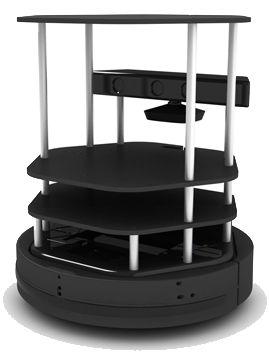
\includegraphics[]{fig/turtlebot_2}
      \end{center}
    \end{column}
  \end{columns}
\end{frame}

\begin{frame}
  \frametitle{System overview}
  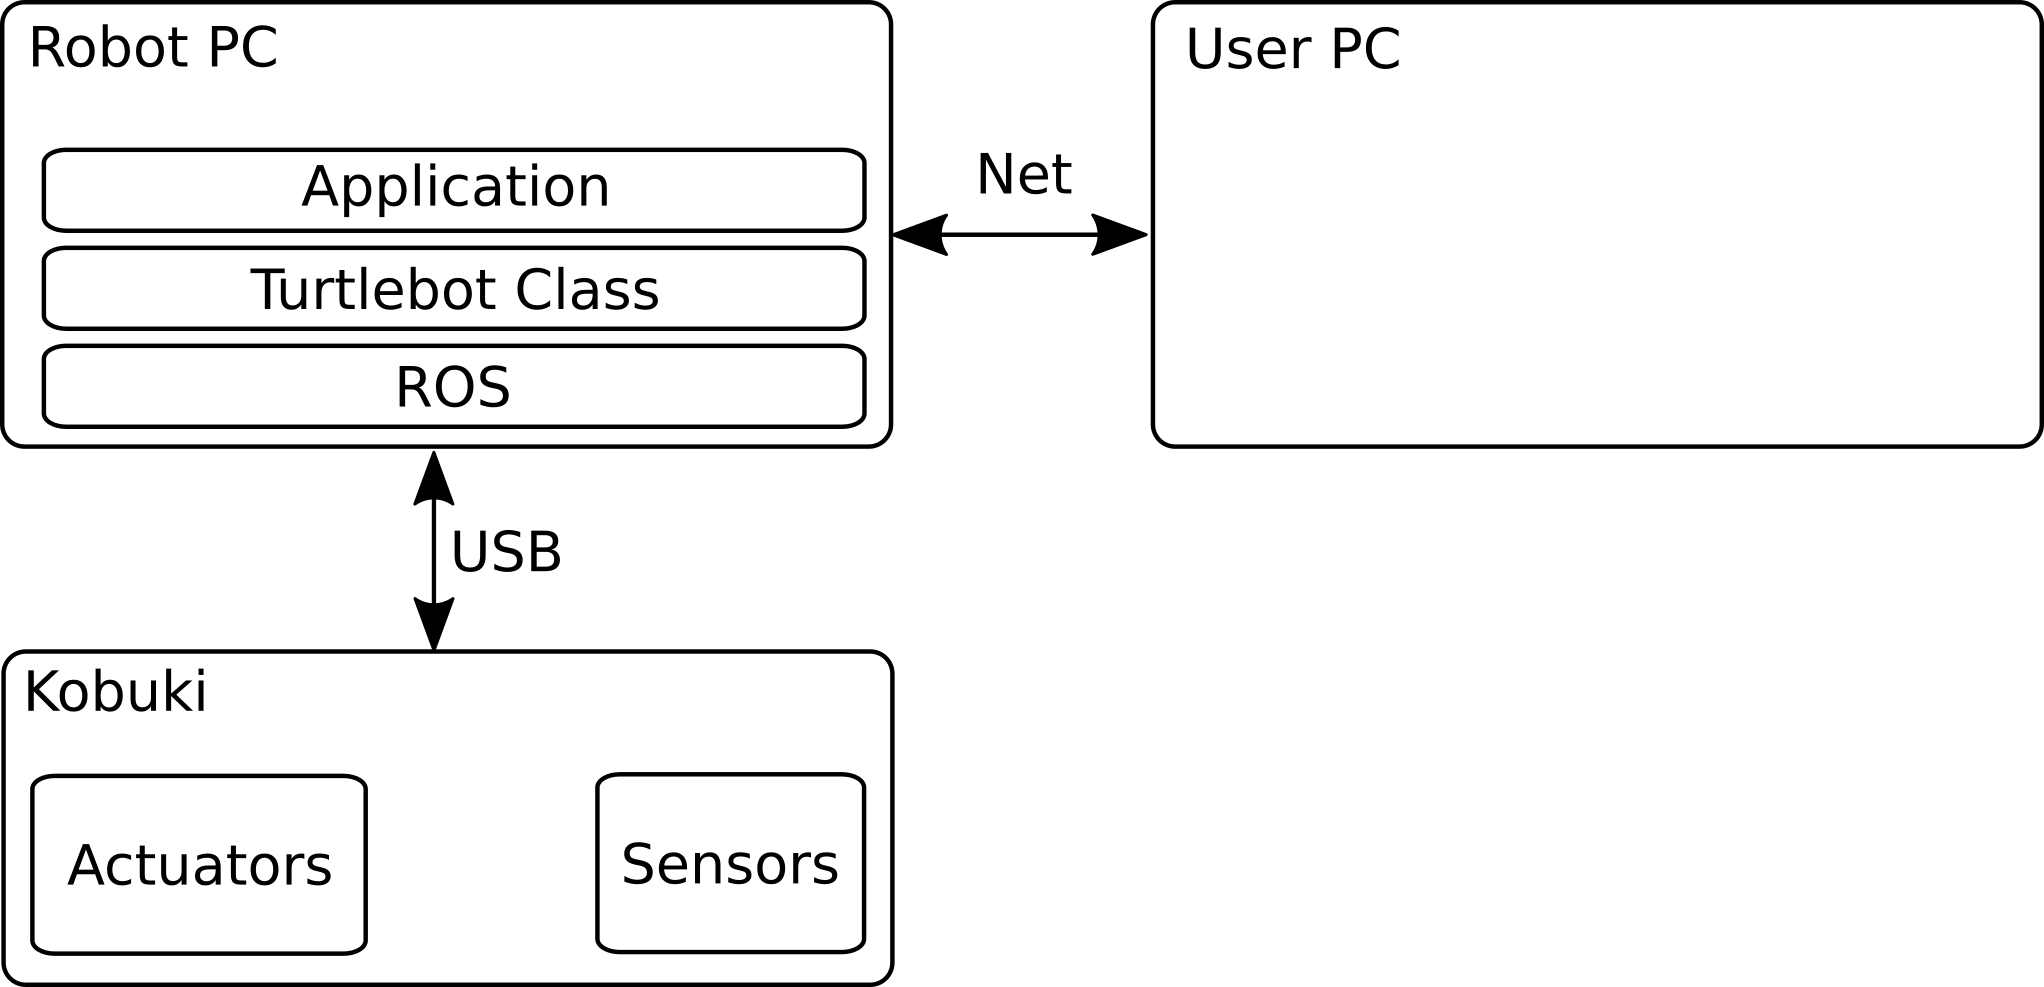
\includegraphics[width=\textwidth]{fig/system}
\end{frame}

\begin{frame}
  \frametitle{Robot Operating System (ROS)}
  \begin{columns}
    \begin{column}{0.5\textwidth}
      \begin{itemize}
      \item Middleware that integrates, sensors, robots and logic into modular system.
      \item In barebones it prowides communication layer between processing units.
      \item Suportsu multiple language and multiple machines.
      \item The main building blocks are Nodes, Topics and Services.
      \end{itemize}
    \end{column}
    \begin{column}{0.5\textwidth}
      \begin{itemize}
      \item Node - buildig block of robotic system. (camera driver, robot controller, image filter ...)
      \item Topic - named stream of data with same type.(rgb camera image, odometry, robot cmd ...)
      \item Service - named function, with specific request and response. (reset odometry, open gripper, compute ik ...)
      \end{itemize}
    \end{column}
  \end{columns}
\end{frame}


\begin{frame}[fragile]
  \frametitle{Turtlebot Python Class}
  \begin{itemize}
  \item
    \verb|cmd_velocity(linear=0, angular=0) -> None|\break commands linear and angular velocity to the robot, this command has to be called repeatedli to ensure that the robot is moving.
  \item
    \verb|get_odometry() -> [x,y,a]|\break get current position, estimated from the encoders and gyroscope.
  \item
    \verb|reset_odometry() -> None|\break sets current position as an origin.
  \end{itemize}
\end{frame}

\begin{frame}[fragile]
  \frametitle{Turtlebot Python Class continue}
  \begin{itemize}
  \item \verb|get_rgb_image() -> image|\break gets RGB image from the RGBD camera.
  \item \verb|get_depth_image() -> image|\break gets depth image from RGBD camera.
  \item \verb|get_point_cloud() -> point_cloud|\break gets pointcloud from RGBD camera.
  \item \verb|get_rgb_K(self) -> K|\break gets calibration matrix K for RGB camera.
  \item \verb|get_depth_K(self) -> K|\break gets calibration matric K for Depth camera.
  \end{itemize}
\end{frame}

\begin{frame}[fragile]
  \frametitle{Turtlebot Python Class continue}
  \begin{itemize}
  \item \verb|register_button_event_cb(fun) -> None|\break register button event callback.
  \item \verb|register_bumper_event_cb(fun) -> None|\break register bumper event callback.
  \item \verb|play_sound(sound_id=0) -> None|\break plays one of the predefined sounds.
  \end{itemize}
\end{frame}

\begin{frame}[fragile]
  \frametitle{Examples: Move straight 1m}
  \inputminted[linenos, numbersep=5pt, frame=lines]{python}{../scripts/example_move_1m.py}
\end{frame}

\begin{frame}[fragile]
  \frametitle{Connect to robots}
   \begin{itemize}
   \item Network in the e210 essid: e210bot, key: j6UsAC8a
   \item Using ssh: \verb|ssh ros@turtle01| pass: r0sr0s
   \item Start robot driver: \verb|turtle_start|
   \item Examples are in \verb|./examples/|
   \item To start one: \verb|python example_move_1m.py|
   \end{itemize}
\end{frame}

\begin{frame}[fragile]
  \frametitle{Resources}
   \begin{itemize}
   \item Turtlebot
     \begin{itemize}
     \item \url{https://gitlab.fel.cvut.cz/wagnelib/turtlebot}
     \item \url{http://www.turtlebot.com/turtlebot2/}
     \item \url{http://wiki.ros.org/Robots/TurtleBot}
     \item \url{http://wiki.ros.org/kobuki}
     \end{itemize}
   \item Python
     \begin{itemize}
     \item \url{https://www.python.org}
     \item \url{https://docs.python.org/2.7/}
     \end{itemize}
   \item ROS
     \begin{itemize}
     \item \url{http://www.ros.org}
     \item \url{http://wiki.ros.org}
     \item \url{https://answers.ros.org}
     \end{itemize}
   \end{itemize}
\end{frame}



\end{document}

